% Set a pdf version and a document type
\ifx\pdfminorversion\undefined\else\pdfminorversion=4\fi
\documentclass[aspectratio=169,t,table]{beamer}

% Import all necessary packages
% Use this file to import all packages which are needed for the lecture
\usepackage[english]{babel}
\usepackage[utf8]{inputenc}
\usepackage[sfdefault]{roboto}
\usepackage[T1]{fontenc}
\usepackage{amsmath,amssymb}
\usepackage{graphicx}
\usepackage{listings}
\usepackage[backend=biber,sorting=none,doi=true,style=ieee]{biblatex}
\usepackage{url}
\usepackage{hyperref}
\usepackage{fontawesome5}
\usepackage{graphicx}
\usepackage{booktabs}
\usepackage{calc}
\usepackage{ifthen}
\usepackage{tabularx}
\usepackage{longtable}
\usepackage{makecell}
\usepackage{multicol}
\usepackage{multirow}
\usepackage{hhline}
\usepackage{qrcode}
\usepackage{xcolor}
\usepackage{cleveref}
\usepackage{tikz}
\usepackage{tikz-cd}
\usepackage{pgfplots,pgfplotstable,pgf-pie}
\usepackage[linesnumbered]{algorithm2e}
\usepackage{array}
\usepackage{mathtools}
\usetikzlibrary{patterns}
\usetikzlibrary{arrows.meta}


% Set the theme (customized FAU beamer theme)
\usetheme[%
	image,%
	longtitle,%
	inst=tf%
]{fau}

% Set all important settings and define commands that are used in more than one lecture
% English version FAU Logo
\usepackage[english]{babel}
% German version FAU Logo
%\usepackage[ngerman]{babel}

\usepackage[utf8]{inputenc}
\usepackage[T1]{fontenc}
\usepackage{amsmath,amssymb}
\usepackage{graphicx}
\usepackage{listings}
\usepackage[backend=biber,sorting=none,doi=true,style=ieee]{biblatex}

% Options:
%  - inst:      Institute
%                 med:      MedFak FAU theme
%                 nat:      NatFak FAU theme
%                 phil:     PhilFak FAU theme
%                 rw:       RWFak FAU theme
%                 rw-jura:  RWFak FB Jura FAU theme
%                 rw-wiso:  RWFak FB WISO FAU theme
%                 tf:       TechFak FAU theme
%  - image:     Cover image on title page
%  - plain:     Plain title page
%  - longtitle: Title page layout for long title
\usetheme[%
	image,%
	longtitle,%
	inst=tf%
]{fau}

% Enable semi-transparent animation preview
\setbeamercovered{transparent}

% Enable frame numbering
%\setbeamertemplate{footline}[frame number]


\lstset{%
	language=Python,
	tabsize=2,
	basicstyle=\tt,
	keywordstyle=\color{blue},
	commentstyle=\color{green!50!black},
	stringstyle=\color{red},
	numbers=left,
	numbersep=0.5em,
	xleftmargin=1em,
	numberstyle=\tt
}

\defbibheading{bibliography}{}
\addbibresource{references.bib}

\date[SS2022]{Summer semester 2022}


\usepackage{url}
\usepackage{enumitem}
\setlist[itemize]{noitemsep, nolistsep}
\setlist[itemize]{label=\footnotesize\raisebox{.275ex}{$\bullet$}}
\usepackage{hyperref}
\usepackage{fontawesome5}
\usepackage{graphicx}
\usepackage{booktabs}
\usepackage{calc}
\usepackage{ifthen}

\usepackage{tabularx}
\usepackage{makecell}

\usepackage{xcolor}
\definecolor{airforceblue}{rgb}{0.36, 0.54, 0.66}
\definecolor{ForestGreen}{rgb}{0.34, 0.139, 0.34}

% English version
\institute[CS6]{Chair of Computer Science 6 (Data Management), Friedrich-Alexander University Erlangen-N\"urnberg}
% German version
% \institute[Lehrstuhl]{Lehrstuhl, Friedrich-Alexander-Universit\"at Erlangen-N\"urnberg}

\setbeamertemplate{section in toc}[sections numbered]

\setbeamertemplate{section page}{%
	\begingroup
	\begin{beamercolorbox}[sep=10pt,center,rounded=true,shadow=true]{section title}
		\usebeamerfont{section title}\thesection~\insertsection\par
	\end{beamercolorbox}
	\endgroup
}

\usepackage{tikz}
\usepackage{tikz-cd}
\usepackage{pgfplots,pgfplotstable,pgf-pie}

\newcommand{\tikzmark}[1]{\tikz[remember picture] \node[coordinate] (#1) {#1};}

\tikzset{
	every overlay node/.style={
			%draw=black,fill=white,rounded corners,
			anchor=north west, inner sep=0pt,
		},
}
% Usage:
% \tikzoverlay at (-1cm,-5cm) {content};
% or
% \tikzoverlay[text width=5cm] at (-1cm,-5cm) {content};
\def\tikzoverlay{%
	\tikz[remember picture, overlay]\node[every overlay node]
}%

\newcommand{\plots}{0.611201}
\newcommand{\plotm}{2.19882}

\newcommand{\MaxNumberX}{3}
\newcommand{\MaxNumberY}{5}

\pgfmathdeclarefunction{gauss}{2}{%
	\pgfmathparse{1/(#2*sqrt(2*pi))*exp(-((x-#1)^2)/(2*#2^2))}%
}

\tikzset{
	thick,
	>=latex,
	every edge/.style={draw=gray, thick, >=latex},
	vertex/.style = {
			circle,
			fill            = black,
			outer sep = 2pt,
			inner sep = 1pt,
		}
}
\usetikzlibrary{matrix,mindmap}
\usetikzlibrary{arrows,decorations.pathmorphing,backgrounds,fit,positioning,shapes.symbols,chains,intersections,snakes}
\tikzset{level 1/.append style={sibling angle=50,level distance = 165mm}}
\tikzset{level 2/.append style={sibling angle=20,level distance = 45mm}}
\tikzset{every node/.append style={scale=1}}
% read in data file
\pgfplotstableread{data/iris.dat}\iris
% get number of data points
\pgfplotstablegetrowsof{\iris}
\pgfmathsetmacro\NumRows{\pgfplotsretval-1}

\usepgfplotslibrary{groupplots}
\pgfplotsset{height=4cm,width=8cm,compat=1.14}

\tikzset{
	vertex/.style = {
			circle,
			fill            = black,
			outer sep = 2pt,
			inner sep = 1pt,
		}
}

\tikzset{
	mynode/.style={
			draw,
			thick,
			anchor=south west,
			minimum width=2cm,
			minimum height=1.3cm,
			align=center,
			inner sep=0.2cm,
			outer sep=0,
			rectangle split,
			rectangle split parts=2,
			rectangle split draw splits=false},
	reverseclip/.style={
			insert path={(current page.north east) --
					(current page.south east) --
					(current page.south west) --
					(current page.north west) --
					(current page.north east)}
		}
}

\tikzset{basic/.style={
			draw,
			rectangle split,
			rectangle split parts=2,
			rectangle split part fill={blue!20,white},
			minimum width=2.5cm,
			text width=2cm,
			align=left,
			font=\itshape
		},
	Diamond/.style={ diamond,
			draw,
			shape aspect=2,
			inner sep = 2pt,
			text centered,
			fill=blue!10!white,
			font=\itshape
		}}


\tikzset{level 1/.append style={sibling angle=50,level distance = 165mm}}
\tikzset{level 2/.append style={sibling angle=20,level distance = 45mm}}
\tikzset{every node/.append style={scale=1}}

\usetikzlibrary{arrows,decorations.pathmorphing,backgrounds,fit,positioning,shapes.symbols,chains,intersections,snakes,positioning,matrix,mindmap,shapes.multipart,shapes,calc,shapes.geometric}



% Title, author(s), and date
\title[KDDmUe~3.~Data]{3. Getting to Know Your Data} %
\subtitle{Knowledge Discovery in Databases with Exercises}
\author[D.~Probst]{Dominik Probst, \texttt{dominik.probst@fau.de}}


% Metadata
\input{x-additional/vc.tex}
\hypersetup{
	pdftitle={KDDmUe - 3. Getting to Know Your Data},
	pdfkeywords={
		KDD, 
		KDDmUe, 
		Knowledge Discovery in Databases, 
		Knowledge Discovery in Databases with Exercises, 
		FAU Erlangen-Nürnberg, 
		Data Science, 
		Machine Learning, 
		Data Mining, 
		Lecture, 
		Data,
		Data Objects,
		Data Types,
		Data Statistical Description,
		Data Visualization,
		Data Similarity,
		Data Understanding,
		Basic Data Analysis,
		Data Exploration,
		Version \GITAbrHash
	},
	pdfsubject={Lecture on data types, statistical descriptors, visualization techniques, and similarity measures to understand, analyze, and compare data.},
	pdfcreator={Dominik Probst, CS6, FAU Erlangen-Nürnberg},
	pdflang={English}
}


% Read in the required data files
\pgfplotstableread{data/iris.dat}\iris
\pgfplotstablegetrowsof{\iris}
\pgfmathsetmacro\NumRows{\pgfplotsretval-1}
\pgfplotstableread{
	10.46365192956
	90.22330318663
	15.4712651178
	80.87219994452
	90.92824632322
	80.69935247007
	170.8222081627
	140.3601041144
	220.9047131581
	80.05005282649
	90.650706465
	170.2352199894
	70.76424153088
	10.370245979
	70.12513239519
	20.64730407495
	70.2072208982
	14.7683650153
	14.0063750733
	19.324137585
	20.40858604381
	18.0368674939
	80.02681240716
	80.26418810694
	120.1941169594
	90.62080674537
	30.24961728242
	30.27316960403
	170.9038479307
	70.40481579419
	10.814441695
	80.40741573499
	60.08031313304
	130.1781459953
	100.206134367
	150.0864695726
	90.03013313987
	40.46906993699
	90.27542593922
	110.387166818
	50.34088290758
	70.35790199406
	110.8693581818
	100.8557924873
	130.969617244
	100.6354692297
	30.03046442179
	60.60358722529
	120.2836888554
	80.46665782108
	130.9221860476
	150.1323993544
	70.16507829073
	50.69317421704
	150.4624253296
	160.9138444234
	60.44259653768
	160.4478862876
	30.46926929558
	100.8862152053
	100.4982459647
	130.079580222
	100.8219448481
	120.1887774019
	20.27608579327
	40.21879129366
	80.6626149873
	30.05616084556
	120.2628717929
	30.07385860151
	120.1834370192
	70.86785100457
	220.3039915506
	70.6084726129
	30.38040559575
	40.77264935147
	130.9493967532
	140.1237678197
	60.79956429934
	80.7032357113
	60.08645967617
	90.19491098171
	17.1651582777
	40.7041931405
	30.78091331321
	50.20247821499
	13.8921717364
	60.09560236506
	18.5811121283
	10.3758110312
	80.95955605147
	12.4511725524
	40.67834498484
	11.0234433275
	15.364443589
	80.23928346825
	60.30079928878
	90.95330967273
	12.5692010856
	11.8362767596
}\datatable
\pgfplotstablesort{\sorted}{\datatable}
\pgfplotstablegetrowsof{\datatable}
\edef\numrows{\pgfplotsretval}


% IMPORTANT: 
% This document requires you to build some figures before you can compile it.
% Execute "make figures" in the main directory to build the figures.
% If you prefer to build the figures manually, you can find the required scripts in the "src" directory.

% Start the document
\begin{document}

% Title
\maketitle

{ % Outline
	\setbeamertemplate{footline}{}
	\begin{frame}[noframenumbering]{Outline}
		\tableofcontents

	\end{frame}
}

% Body
\section{Data Objects and Attribute Types}

\begin{frame}{Types of Data Sets}
	\begin{columns}
		\begin{column}{0.45\textwidth}
			\textbf{Records:}
			\begin{itemize}
				\item Relational records.
				\item Data matrix, e.g. numerical matrix, crosstabs.
				\item Document data: text documents, typically represented as
				      \textit{term-frequency vectors}. \tikzmark{n1}
				\item \textit{Transaction data}. \tikzmark{n2}
			\end{itemize}
			\textbf{Graph and network:}
			\begin{itemize}
				\item World wide web.
				\item Social information networks.
				\item Molecular structures.
			\end{itemize}
		\end{column}

		\begin{column}{0.45\textwidth}  %%<--- here
			\begin{table}
				\begin{tabular}{|c|c|c|c|c|c|c|}
					\multicolumn{1}{c|}{}  & \rotatebox[origin=c]{270}{team} & \rotatebox[origin=c]{270}{couch} & \rotatebox[origin=c]{270}{play} & \rotatebox[origin=c]{270}{ball} & \rotatebox[origin=c]{270}{score} & \rotatebox[origin=c]{270}{game} \\ \hline
					\tikzmark{t1}Document1 & 3                               & 0                                & 5                               & 0                               & 2                                & 6                               \\ \hline
					Document2              & 0                               & 7                                & 0                               & 2                               & 1                                & 0                               \\ \hline
					Document3              & 0                               & 1                                & 0                               & 0                               & 1                                & 2                               \\
					\hline
				\end{tabular}\\[0.5cm]
				\begin{tabular} { | c | l |}
					\hline
					\textbf{TID}   & \textbf{Items}             \\
					\hline
					\tikzmark{t2}1 & Bread, Coke, Milk          \\\hline
					2              & Beer, Bread                \\\hline
					3              & Beer, Coke, Diapers, Milk  \\\hline
					4              & Beer, Bread, Diapers, Milk \\\hline
					5              & Coke, Diapers, Milk        \\
					\hline
				\end{tabular}
			\end{table}
			\begin{tikzpicture}[remember picture,overlay]
				\draw[faucyan,thick,->] ([yshift=1mm]n1) to[out=0,in=180] ([yshift=1mm]t1);
				\draw[faucyan,thick,->] ([yshift=1mm]n2) to[out=0,in=180] ([yshift=1mm]t2);
			\end{tikzpicture}
		\end{column}
	\end{columns}
\end{frame}

\begin{frame}{Types of Data Sets}
	\textbf{Ordered data:}
	\begin{itemize}
		\item Video data: sequences of images.
		\item Temporal data: time series.
		\item Sequential data: transaction sequences.
		\item Genetic sequence data.
	\end{itemize}
	\textbf{Spatial, image and multimedia:}
	\begin{itemize}
		\item Spatial data: maps.
		\item Image data.
		\item Video data.
	\end{itemize}
	% TODO: Add example visualizations:
	% - time series: studends enrolled at FAU (https://www.erlangen.de/desktopdefault.aspx/tabid-1917/4223_read-7988/)
	% - image data: pictures of FAU headquarters and tech fak building as an example for landmarks
\end{frame}

\begin{frame}{Important Characteristics of Structured Data}
	\textbf{Dimensionality}:\\
	Curse of dimensionality (sparse high-dimensional data spaces).\\[0.2cm]
	% make the example with the volume of a cube

	\textbf{Sparsity}:\\
	Only presence counts.\\[0.2cm]

	\textbf{Resolution}:\\
	Patterns depend on the scale.\\[0.2cm]

	\textbf{Distribution}:\\
	Centrality and dispersion.
\end{frame}

\begin{frame}{Data Objects}
	\begin{block}{Data Object}
		A data set consists of data objects. A single \textit{data object} represents an entity.
	\end{block}

	Also known as: Samples, examples, instances, data points, objects, tuples.\\\medskip

	Examples:
	\begin{itemize}
		\item Sales database: customers, store items, sales.
		\item Medical database: patients, treatments.
		\item University database: students, professors, courses.
	\end{itemize}

	\textbf{Data objects are described by attributes}:
	\begin{itemize}
		\item Database rows $\rightarrow$ data objects.
		\item Columns $\rightarrow$ attributes.
	\end{itemize}
\end{frame}

\begin{frame}{Attributes}
	\begin{block}{Attribute}
		An \textit{attribute} represents a specific characteristic such as customer
		unique identifier, customer name, and customer address.
	\end{block}

	Also known as: variable, feature, field, dimension.\\\medskip

	\note[itemize]{
		\item \textit{dimension}: used in DWH, but also in statistics: number of
		observations not number of attributes/variables
		\item \textit{feature}: common in Machine Learning
		\item \textit{variable}: prefered by statisticians
	}

	\begin{itemize}
		\item \textit{Observations}: Observed or measured values of an attribute.
		\item An \textit{attribute vector} or \textit{feature vector} describes a
		      data object by its set of attribtues.
		\item Data sets with one attribute are referred to as \textit{univariate},
		      whereas a \textit{multivariate} data set consists of more than one
		      attribute.
	\end{itemize}
\end{frame}

\begin{frame}{Types of Attributes}
	Two different views:

	\vspace*{1em}
	\begin{columns}[t]
		\begin{column}{0.5\columnwidth}
			\centering
			\begin{tikzpicture}[
					every path/.style={
							thick,
							>=latex,
							rounded corners=5pt,
							draw,
							->
						},
					every edge/.style={draw, thick, >=latex},
					box/.style={
							draw,
							fill=white,
							rounded corners=.25em,
							% text height=.8em,
							outer sep=0,
							inner sep=.6em,
							align=center
						}
				]
				\node[box] at (0,0) (root) {Types of Measurements};
				\node[box, below left=2em and -3em of root] (qualitative) {Qualitative};
				\node[box, below right=2em and -3em of root] (quantitative) {Quantitative};

				\node[box, below left=2em and -2.5em of qualitative] (nominal) {Nominal};
				\node[box, below right=2em and -2.5em of qualitative] (ordinal) {Ordinal};

				\node[box, below left=2em and -2.5em of quantitative] (interval) {Interval};
				\node[box, below right=2em and -2.5em of quantitative] (ratio) {Ratio};

				\coordinate[below=1em of root.south] (root-below);
				\coordinate[above=1em of quantitative.north] (quantitative-above);
				\coordinate[above=1em of qualitative.north] (qualitative-above);
				\path[faugray] (root.south) -- (root-below) -- (qualitative-above) -- (qualitative.north);
				\path[faugray] (root.south) -- (root-below) -- (quantitative-above) -- (quantitative.north);

				\coordinate[below=1em of quantitative.south] (quantitative-below);
				\coordinate[above=1em of interval.north] (interval-above);
				\coordinate[above=1em of ratio.north] (ratio-above);
				\path[faugray] (quantitative.south) -- (quantitative-below) -- (interval-above) -- (interval.north);
				\path[faugray] (quantitative.south) -- (quantitative-below) -- (ratio-above) -- (ratio.north);

				\coordinate[below=1em of qualitative.south] (qualitative-below);
				\coordinate[above=1em of nominal.north] (nominal-above);
				\coordinate[above=1em of ordinal.north] (ordinal-above);
				\path[faugray] (qualitative.south) -- (qualitative-below) -- (nominal-above) -- (nominal.north);
				\path[faugray] (qualitative.south) -- (qualitative-below) -- (ordinal-above) -- (ordinal.north);
			\end{tikzpicture}
		\end{column}

		\begin{column}{0.5\columnwidth}
			\centering
			\begin{tikzpicture}[
					every path/.style={
							thick,
							>=latex,
							rounded corners=5pt,
							draw,
							->
						},
					every edge/.style={draw, thick, >=latex},
					box/.style={
							draw,
							fill=white,
							rounded corners=.25em,
							% text height=.8em,
							outer sep=0,
							inner sep=.6em,
							align=center
						}
				]
				\node[box] at (0,0) (root) {Types of Attributes};
				\node[box, below left=2em and -2em of root] (categorical) {Categorical};
				\node[box, below right=2em and -2em of root] (numerical) {Numerical};
				\node[box, below left=2em and -2em of numerical] (continuous) {Continuous};
				\node[box, below right=2em and -2em of numerical] (discrete) {Discrete};

				\coordinate[below=1em of root.south] (root-below);
				\coordinate[above=1em of categorical.north] (categorical-above);
				\coordinate[above=1em of numerical.north] (numerical-above);
				\path[faugray] (root.south) -- (root-below) -- (categorical-above) -- (categorical.north);
				\path[faugray] (root.south) -- (root-below) -- (numerical-above) -- (numerical.north);

				\coordinate[below=1em of numerical.south] (numerical-below);
				\coordinate[above=1em of continuous.north] (continuous-above);
				\coordinate[above=1em of discrete.north] (discrete-above);
				\path[faugray] (numerical.south) -- (numerical-below) -- (continuous-above) -- (continuous.north);
				\path[faugray] (numerical.south) -- (numerical-below) -- (discrete-above) -- (discrete.north);
			\end{tikzpicture}
		\end{column}
	\end{columns}
	\vspace*{1em}
	\begin{itemize}
		\item \textit{Qualitative} measurements describe an attribute without
		      providing a size or quantity.

		\item \textit{Quantitative} measurements, often also called \textit{numerical}
		      attributes, are quantitatively measured and often represented in integers or
		      real values.
	\end{itemize}
\end{frame}



\begin{frame}{Attribute Types}
	\textbf{Nominal}:
	\begin{itemize}
		\item Categories, states, or "names of things".
		\item E.g. \texttt{hair\_color} $= \{\text{auburn, black, blond, brown, grey, red, white}\}$.
		\item Other examples: \texttt{marital\_status}, \texttt{occupation}, \texttt{ID}, \texttt{ZIP code}.
	\end{itemize}

	\textbf{Binary}:
	\begin{itemize}
		\item Nominal attribute with only two states ($0$ and $1$).
		\item \textbf{Symmetric binaries}: both outcomes equally important, such as \texttt{sex}.
		\item \textbf{Asymmetric binary}: outcomes not equally important. \\
		      E.g. medical test (positive vs. negative).\\
		      Convention: assign 1 to most important outcome (e.g. diabetes, HIV positive).
	\end{itemize}

	\textbf{Ordinal}:
	\begin{itemize}
		\item Values have a meaningful order (ranking), but magnitude between
		      successive values is not known.
		\item E.g. \texttt{size} $= \{\text{small, medium, large}\}$, grades, army rankings.
	\end{itemize}
\end{frame}

\begin{frame}{Numerical Attribute Types}
	\begin{columns}[t]
		\begin{column}{0.5\columnwidth}
			\centering \textbf{Interval-Scaled Attributes}
			\begin{itemize}
				\item Measured on a scale of \textbf{equally sized} units.
				\item No true zero-point.
				\item Values have order.
				\item E.g. temperature in $C$ or $F$, calender dates.
			\end{itemize}
		\end{column}
		\begin{column}{0.5\columnwidth}
			\centering \textbf{Ratio-Scaled Attributes}
			\begin{itemize}
				\item Inherent \textbf{zero point}.
				\item We can speak of values as being an order of magnitude larger
				      than the unit of measurement.
				\item E.g. temperature in Kelvin, length, counts, monetary quantities.
			\end{itemize}
		\end{column}
	\end{columns}

	\vspace*{1em}
	\begin{tikzpicture}[xscale=0.032]
		\def\Tzero{-273.15}  % absolute zero
		\def\Tnitro{-195.79} % liquid nitrogen
		\def\Tbody{36.8}     % body temperature
		\def\Tboil{100}      % boiling temperature
		\def\Tmax{140}       % maximum temperature on the scale
		\def\h{0.5}         % axis off sets
		\def\tick####1####2####3{\draw[thick,####3] (####1+.08) --++ (0,-.16) node[below=-.5pt,scale=1] {\scriptsize ####2};}
		\def\Ts####1{{25+50/(\Tmax-\Tzero)*(####1-\Tzero)}} % convert temperature to [25,50] range

		% AXIS
		\draw[->,thick] % degrees Celsius
		(1.02*\Tzero,0) -- (1.1*\Tmax,0) node[right] {$^\circ$C};
		\draw[->,thick] % Kelvin
		(1.02*\Tzero,-\h) -- (1.1*\Tmax,-\h) node[right] {K};
		\draw[->,thick] % Fahrenheit
		(1.02*\Tzero,-2*\h) -- (1.1*\Tmax,-2*\h) node[right] {$^\circ$F};

		% LABEL
		\node[above=-0.2em,align=center] at (\Tzero,0.1) {\scriptsize absolute\\[-2]\strut \scriptsize zero};
		\node[above=-0.2em,align=center] at (\Tnitro,0.1) {\scriptsize liquid\\[-2]\strut \scriptsize nitrogen};
		\node[left=4,above=-0.2em,align=center] at (0,0.1) {\scriptsize water\\[-2]\strut \scriptsize freezes};
		\node[right=4,above=-0.2em,align=center] at (\Tbody,0.1) {\scriptsize human\\[-2]\strut \scriptsize body};
		\node[above=-0.2em,align=center] at (\Tboil,0.1) {\scriptsize water\\[-2]\strut \scriptsize boils};

		% CELSIUS
		\tick{\Tzero,0}{$-273.15$}{faublue} % absolute zero
		\tick{\Tnitro,0}{\hspace{6pt}$-195.79$}{faublue} % liquid nitrogen
		\tick{0,0}{0}{faublue}              % freezing temperature
		\tick{\Tbody,0}{36.8}{faugreendark}            % body temperature
		\tick{\Tboil,0}{100}{faured}        % boiling temperature

		% KELVIN
		\tick{\Tzero,-\h}{0}{faublue}   % absolute zero
		\tick{\Tnitro,-\h}{77}{faublue}           % liquid nitrogen
		\tick{0,-\h}{273.15}{faublue}       % freezing temperature
		\tick{\Tbody,-\h}{310.0}{faugreendark}        % body temperature
		\tick{\Tboil,-\h}{373.15}{faured}   % boiling temperature

		% FAHRENHEIT
		\tick{\Tzero,-2*\h}{$-459.67$}{faublue} % absolute zero
		\tick{\Tnitro,-2*\h}{$-320$}{faublue}      % liquid nitrogen
		\tick{0,-2*\h}{32}{faublue}          % freezing temperature
		\tick{\Tbody,-2*\h}{98.2}{faugreendark}         % body temperature
		\tick{\Tboil,-2*\h}{212}{faured}     % boiling temperature
	\end{tikzpicture}
\end{frame}

\begin{frame}[c]{Continuous vs. Discrete Attributes}
	\begin{columns}[t]
		\begin{column}{0.5\columnwidth}
			\centering \textbf{Continuous Attributes}
			\begin{itemize}
				\item Has real numbers as attribute values.\\
				      E.g. temperature, height, or weight.
				\item Practically, real values can only be measured and represented using a finite number of digits.
				\item Continuous attributes are typically represented as floating-point variables.
			\end{itemize}
		\end{column}
		\begin{column}{0.5\columnwidth}
			\centering \textbf{Discrete Attributes}
			\begin{itemize}
				\item Has finite or countably infinite elements.\\
				      E.g. ZIP code, profession, or the set of words in a collection of documents.
				\item Sometimes represented as integer variables.
				      % \item Note: Binary attributes are a special case of discrete attributes.
			\end{itemize}
			\begin{alertblock}{Note}
				Binary attributes are a special case of discrete attributes.
			\end{alertblock}
		\end{column}
	\end{columns}
\end{frame}

\section{Basic Statistical Descriptors of Data}

\begin{frame}{Basic Statistical Descriptions of Data}
	\textbf{Motivation}:
	\begin{itemize}
		\item To better understand the data: central tendency, variation and spread.
	\end{itemize}

	\textbf{Data dispersion characteristics}:
	\begin{itemize}
		\item Median, max, min, quantiles, outliers, variance etc.
	\end{itemize}

	\textbf{Numerical dimensions correspond to sorted intervals.}\\
	\begin{itemize}
		\item Data dispersion: analyzed with multiple granularities of precision.
		\item Boxplot or quantile analysis on sorted intervals
	\end{itemize}

	\textbf{Dispersion analysis on computed measures.}\\
	\begin{itemize}
		\item Folding measures into numerical dimensions.
		\item Boxplot or quantile analysis on the transformed cube.
	\end{itemize}
\end{frame}

\begin{frame}{Population vs. Sample}
	\begin{columns}[t]
		\begin{column}{0.5\columnwidth}
			\centering \textbf{Population}
			\begin{itemize}
				\item Collection of \textit{all} data objects of interest.\\ E.g. all
				      people currently living in Germany or all enrolled students at FAU.
				\item Population size often denoted by $N$.
				\item Hard to define and to observe.\\E.g. a survey requiring all enrolled
				      students is often not feasible as not all will participate.
			\end{itemize}
			\begin{alertblock}{Note}
				Unlikely that we have data of a whole population. Thus, we can assume we
				always have a sample.
			\end{alertblock}
		\end{column}
		\begin{column}{0.5\columnwidth}
			\centering \textbf{Sample}
			\begin{itemize}
				\item Randomly selected and representative subset of a population obtained
				      by a sampling method\footnote[frame]{Example include but not limited to
					      simple random sampling, stratified sampling.}.
				\item Sample size often denoted by $n$.
				\item Sample guards against (unconscious) investigator biases.
				\item Samples are faster and less costly to obtain.
				\item More control regarding (missing) values and outlier.
			\end{itemize}
		\end{column}
	\end{columns}
\end{frame}

\begin{frame}{Measuring the Central Tendency: Mean and Trimmed Mean}
	\begin{columns}
		\begin{column}{0.5\textwidth}
			\textbf{Arithmetic Mean}

			Simple and most commonly used measure of central tendency:

			\begin{equation*}
				\bar{x} = \frac{1}{n} \sum_{i=1}^{n} x_i.
			\end{equation*}

			\begin{itemize}
				\item Sensitive to extreme values (outliers).
			\end{itemize}
		\end{column}
		\begin{column}{0.5\textwidth}
			\textbf{Trimmed Mean}

			Simple and robust variation of the arithmetic mean:
			\begin{equation*}
				\bar{x} = \frac{x_{([n\alpha]+1)}+ \dots x_{(n-[n\alpha])}}{n-2[n\alpha]}
			\end{equation*}
			where $[n\alpha]$ denotes the greatest index less than or equal to $n\alpha$. In other words:

			\begin{itemize}
				\item Order data.
				\item Discard lowest $100\alpha\%$ and highest $100\alpha\%$.
				\item Compute arithmetic mean on remaining data.
			\end{itemize}


			Note: 50\% trimmed mean corresponds to median.
		\end{column}
	\end{columns}
\end{frame}

\begin{frame}{Measuring the Central Tendency: Median (I)}
	The \textbf{median} $\tilde{x}$ is the middle value of ordered observations where
	\begin{itemize}
		\item A minimum of 50\% of all values are lesser or equal $\tilde{x}$.
		\item A minimum of 50\% of all values are greater or equal $\tilde{x}$.
	\end{itemize}

	\begin{align*}
		\tilde{x} = %
		\begin{cases}
			x_{\frac{N}{2}}                               & \text{if $N$ mod $2 = 0$,}    \\
			\frac{x_{\frac{N-1}{2}}+x_{\frac{N+1}{2}}}{2} & \text{if $N$ mod $2 \neq 0$.}
		\end{cases}
	\end{align*}
	More robust compared to mean as extreme values does not have such drastic affects.
\end{frame}

\begin{frame}{Measuring the Central Tendency: Median (II)}
	\textbf{Median for interval grouped data} (An Example)
	\begin{table}
		\begin{tabularx}{\textwidth}{|c|c|p{4.5em}|X|X|X|}
			\rowcolor{faugray!62}\textbf{Class $i$} & \textbf{Age $x_i$} ($x_i^l$ - $x_i^u$) & \textbf{Class Width $\Delta_i$} & \textbf{Absolute\newline Frequency $n_i$} & \textbf{Relative\newline Frequency $f_i$} & \textbf{Cummulative rel.\newline Frequency $F_i$} \\ \hline
			$1$                                     & $1-5$                                  & 4                               & $200$                                     & 0.06262                                   & 0.06262                                           \\
			$2$                                     & $6-15$                                 & 9                               & $450$                                     & 0.14089                                   & 0.20351                                           \\
			$3$                                     & $16-20$                                & 4                               & $300$                                     & 0.09393                                   & 0.29743                                           \\
			\rowcolor{fauyellow!62} $4$             & $21-50$                                & 29                              & $1500$                                    & 0.46963                                   & 0.76706                                           \\
			$5$                                     & $51-80$                                & 29                              & $700$                                     & 0.21916                                   & 0.98622                                           \\
			$6$                                     & $81-110$                               & 29                              & $44$                                      & 0.01378                                   & 1.00000                                           \\ \hline
			$\sum$                                  &                                        &                                 & 3194                                      & 1.00000                                   &                                                   \\ \hline
		\end{tabularx}
	\end{table}

	Median lies between the fourth group, that is within the age group of 21 to 50 years.
\end{frame}

\begin{frame}{Measuring the Central Tendency: Median (III)}
	\textbf{Median for interval grouped data}

	For grouped data we typically have no information about the underlying
	distribution. However, we can assume that the data is equally
	distributed. In this case we can approximate the median with the following
	steps:
	\begin{itemize}
		\item Order data (in our example by age, not by frequencies!).
		\item Compute relative frequencies, that is: frequency divided by sum of all frequencies.
		\item Compute cummulative relative frequencies.
	\end{itemize}

	Determine median with these considerations:
	\begin{itemize}
		\item $F_i=0.5$: We have no clear median. Therefore: Take this class ($F_i=0.5$) and the next one ($F_i > 0.5$) to obtain the median.
		\item $F_i>0.5$: Median lies within the class where the cummulative
		      relative frequency exceeds 50\% for the first time. Compute the approximate median with:
	\end{itemize}
\end{frame}

\begin{frame}{Measuring the Central Tendency: Median (IV)}
	\textbf{Median for interval grouped data}

	$F_i>0.5$: Median lies within the class where the cummulative
	relative frequency exceeds 50\% for the first time. Compute the approximate median with:
	\begin{align*}
		\tilde{x} \approx x_i^l +\left(\frac{\frac{1}{2}\sum_{i=1}^{N}n_i - \sum_{k=1}^{N-1} n_k}{n_i}\right)\Delta_i
	\end{align*}
	where
	\begin{itemize}
		\item $i$ denotes the class number in which the median lies,
		\item $x_i^l$ is the lower boundary,
		\item $\sum_{i=1}^{N}n_i$ is the sum of all absolute frequencies,
		\item $\sum_{k=1}^{N-1} n_k$ is the cummulative sum of absolute frequencies below class $i$, and
		\item $\Delta_i=x_i^u - x_i^l$ the class width.
	\end{itemize}

	In our example: $\tilde{x} \approx 21 +\left(\frac{\frac{3194}{2} - 950}{1500}\right)*29 \approx 33.51$, i. e. 33 years and 6 months
\end{frame}

\begin{frame}{Measuring the Central Tendency: Mode}
	\textbf{Mode}
	\begin{itemize}
		\item Value that occurs most frequently within the data set.
		\item Can be unimodal, bimodal, multimodal.
		\item Also possible that no mode exists when each value is unique,
		      i. e. occurs only once.
		\item Empirical formula for unimodal modes:
		      \begin{align}
			      \overline{x} - \text{mode} \approx 3(\overline{x}- \tilde{x}).
		      \end{align}
	\end{itemize}
\end{frame}

\begin{frame}{Example of Mode, Median and Mean (I)}
	\begin{columns}[t]
		\begin{column}{0.5\textwidth}
			\vspace{-1em}
			\textbf{Normal distribution}

			\begin{align*}
				f(x \vert \mu, \sigma) = \frac{1}{\sqrt{2\pi\sigma^2}} \exp\left( - \frac{(x-\mu)^2}{2\sigma^2}\right)
			\end{align*}

			\vspace{1em}

			\begin{tikzpicture}[font=\sffamily,
					declare function={Gauss(\x,\y,\z,\u)=1/(\z*sqrt(2*pi))*exp(-((\x-\y+\u*(\x-\y)*sign(\x-\y))^2)/(2*\z^2));},
					every path/.style={
							>=latex,
							rounded corners=3pt,
							draw,
						},
					every pin edge/.style={latex-,line width=1.5pt},
					every pin/.style={fill=yellow!50,rectangle,rounded corners=3pt,font=\small}]
				\begin{axis}[
						every axis plot post/.append style={
								mark=none,samples=101},
						clip=false,
						axis y line=none,
						axis x line*=bottom,
						ymin=0,
						xtick=\empty,]
					\addplot[line width=1.5pt,faucyandark,domain=-3:3] {gauss(0,1)};
					\draw[line width=1.5pt,dashed, black] (0,0) -- (0,0.4);
					% \draw[line width=1.5pt,dashed, fauorange] (0,0) -- (0.6,{Gauss(0.6,0,0.6,-0.4)});
					% \draw[line width=1.5pt,dashed, fauorange] (0,0) -- (1.2,{Gauss(0.5,0,0.7,0.5)});
					\path (1.2,0) coordinate (ML) (0.6,0) coordinate (MR) (0,0) coordinate (MM);
				\end{axis}
				\node[below=2em of MM] (median) {Median};
				\node[right=0em of median] (mean) {Mean};
				\node[right=0em of mean] (mode) {Mode};

				\coordinate[above=0.7em of median.north] (median-above);
				\coordinate[above=0.7em of mean.north] (mean-above);
				\coordinate[above=0.7em of mode.north] (mode-above);

				\path[faugraydark, ->,thick] (mode.north) -- (mode-above) -- (median-above) -- (MM);
				\path[faugraydark, ->,thick] (mean.north) -- (mean-above) -- (median-above) -- (MM);
				\path[faugraydark, ->,thick] (median.north) -- (MM);
			\end{tikzpicture}
		\end{column}
		\begin{column}{0.5\textwidth}
			\textbf{Positively Skewed Data Distribution}
			\begin{tikzpicture}[font=\sffamily,
					declare function={Gauss(\x,\y,\z,\u)=1/(\z*sqrt(2*pi))*exp(-((\x-\y+\u*(\x-\y)*sign(\x-\y))^2)/(2*\z^2));},
					every path/.style={
							>=latex,
							rounded corners=3pt,
							draw,
						},
					every pin edge/.style={latex-,line width=1.5pt},
					every pin/.style={fill=yellow!50,rectangle,rounded corners=3pt,font=\small}]
				\begin{axis}[%
						name=left,
						every axis plot post/.append style={
								mark=none,
								samples=101
							},
						clip=false,
						axis y line=none,
						axis x line*=bottom,
						ymin=0,
						xtick=\empty,
						legend pos=north east,
						% (so the legend looks a bit better)
						legend cell align=left,
						legend style={nodes={scale=0.75, transform shape}}
					]
					\addplot[line width=1.5pt,dashed, black] coordinates {(0.4,0) (0.4,{Gauss(0.4,0.4,0.6,-0.4)})};
					\addplot[line width=1.5pt,dashdotdotted, fauorange] coordinates {(0.8,0) (0.8,{Gauss(0.8,0.4,0.6,-0.4)})};
					\addplot[line width=1.5pt,dotted, faugreendark] coordinates {(1.2,0) (1.2,{Gauss(1.2,0.4,0.6,-0.4)})};
					\addplot[line width=1.5pt,faucyandark,domain=-1.5:3.8] {Gauss(x,0.4,0.6,-0.4)};

					% \draw[line width=1.5pt,dashed, black] (0.4,0) -- (0.4,{Gauss(0.4,0.4,0.6,-0.4)});
					% \draw[line width=1.5pt,dashdotdotted, fauorange] (0.8,0) -- (0.8,{Gauss(0.8,0.4,0.6,-0.4)});
					% \draw[line width=1.5pt,dotted, faugreendark] (1.2,0) -- (1.2,{Gauss(1.2,0.4,0.6,-0.4)});
					\addlegendentry{Median}
					\addlegendentry{Mode}
					\addlegendentry{Mean}
				\end{axis}
			\end{tikzpicture}

			\textbf{Nevatively Skewed Data Distribution}
			\begin{tikzpicture}[font=\sffamily,
					declare function={Gauss(\x,\y,\z,\u)=1/(\z*sqrt(2*pi))*exp(-((\x-\y+\u*(\x-\y)*sign(\x-\y))^2)/(2*\z^2));},
					every path/.style={
							>=latex,
							rounded corners=3pt,
							draw,
						},
					every pin edge/.style={latex-,line width=1.5pt},
					every pin/.style={fill=yellow!50,rectangle,rounded corners=3pt,font=\small}]
				\begin{axis}[%
						name=right,
						every axis plot post/.append style={
								mark=none,samples=101},
						clip=false,
						axis y line=none,
						axis x line*=bottom,
						ymin=0,
						xtick=\empty,
					]
					\addplot[line width=1.5pt,dashed, black] coordinates {(-0.4,0) (-0.4,{Gauss(-0.4,-0.4,0.6,0.4)})};
					\addplot[line width=1.5pt,dashdotdotted, fauorange] coordinates {(-0.8,0) (-0.8,{Gauss(-0.8,-0.4,0.6,0.4)})};
					\addplot[line width=1.5pt,dotted, faugreendark] coordinates {(-1.2,0) (-1.2,{Gauss(-1.2,-0.4,0.6,0.4)})};
					\addplot[line width=1.5pt,faucyandark,domain=-3.8:1.5] {Gauss(x,-0.4,0.6,0.4)};
					% \addlegendentry{Distribution}
				\end{axis}
			\end{tikzpicture}
		\end{column}
	\end{columns}
\end{frame}


\begin{frame}{Properties of Normal Distribution Curves}
	\begin{itemize}
		\item \textbf{The normal distribution:}
		      \begin{itemize}
			      \item From $\mu - \sigma$ to $\mu + \sigma$: contains about $68\%$ of the measurements.
			            \begin{itemize}
				            \item $\mu$: mean,
				            \item $\sigma$: standard deviation.
			            \end{itemize}
			      \item From $\mu - 2 \sigma$ to $\mu + 2\sigma$: contains about $95\%$ of the surface under the curve.
			      \item $\mu-3\sigma$ to $\mu + 3\sigma$: contains about $99.7\%$ of the surface under the curve.
		      \end{itemize}
	\end{itemize}
	\vspace{0.2cm}
	\centering
	\begin{tikzpicture}
		\begin{axis}[
				no markers,
				domain=-3:3,
				samples=100,
				axis lines*=left,
				xlabel=$x$,
				ylabel=$y$,
				height=3.5cm,
				width=5cm,
				xtick={-3,-2,-1,0,1,2,3},
				ytick=\empty,
				enlargelimits=false,
				clip=false,
				% axis on top,
				grid=major
			]
			\addplot [fill=faucyan!62, draw=none, domain=-1:1] {gauss(0,1)} \closedcycle;
			\addplot [very thick,faucyandark] {gauss(0,1)};
			\node[below] at (0,0.15) {$\approx 66 \%$};
		\end{axis}
	\end{tikzpicture}
	\hspace{0.2cm}
	\begin{tikzpicture}
		\begin{axis}[
				no markers,
				domain=-3:3,
				samples=100,
				axis lines*=left,
				xlabel=$x$,
				ylabel=$y$,
				height=3.5cm,
				width = 5cm,
				xtick={-3,-2,-1,0,1,2,3},
				ytick=\empty,
				enlargelimits=false,
				clip=false,
				% axis on top=false,
				grid=major
			]
			\addplot [fill=faucyan!62, draw=none, domain=-2:2] {gauss(0,1)} \closedcycle;
			\addplot [very thick,faucyandark] {gauss(0,1)};
			\node[below] at (0,0.15) {$\approx 95 \%$};
		\end{axis}
	\end{tikzpicture}
	\hspace{0.2cm}
	\begin{tikzpicture}
		\begin{axis}[
				no markers,
				domain=-3:3,
				samples=100,
				axis lines*=left,
				xlabel=$x$,
				ylabel=$y$,
				height=3.5cm,
				width=5cm,
				xtick={-3,-2,-1,0,1,2,3},
				ytick=\empty,
				enlargelimits=false,
				clip=false,
				% axis on top,
				grid = major
			]
			\addplot [fill=faucyan!62, draw=none, domain=-2.97:2.97] {gauss(0,1)} \closedcycle;
			\node[below] at (0,0.15) {$\approx 99.7 \%$};
			\addplot [very thick,faucyandark] {gauss(0,1)};

		\end{axis}
	\end{tikzpicture}
	\hspace{0.2cm}
\end{frame}


\begin{frame}{Measuring the Dispersion of Data (I)}
	\textbf{Variance $\sigma^2$ and standard deviation $\sigma$}:
	\begin{itemize}
		\item Empirical sample variance is the mean: $\overline{\sigma^2} = \frac{1}{n-1} \sum_{i=1}^{n}(x_i-\overline{x})^2$
		\item Standard deviation is the square root $\sigma = \sqrt{\sigma^2}$.
	\end{itemize}
\end{frame}

\begin{frame}{Measuring the Dispersion of Data (II)}
	\begin{itemize}
		\item \textbf{Range} is the difference between the largest and smallest value.
		\item \textbf{Quartiles:} Also known as \textit{quantiles}. Generalization of the median. Median is the $50^{\text{th}}$ quartile.\\
		      Other comon quartiles include $Q_1$ ($25^{\text{th}}$ percentile) and $Q_3$
		      ($75^{\text{th}}$ percentile).\\\smallskip Quartile with order $p$ with
		      ($0 < p < 1$) have following characteristics:
		      \begin{itemize}
			      \item A minimum of $p * 100\%$ of values are lesser or equal to $Q_p$.
			      \item A minimum of $(1 - p) * 100\%$ of values are greater or equal $Q_p$.
		      \end{itemize}
		\item \textbf{Inter quartile range:} IQR $=Q_3-Q_1$.
		\item \textbf{Five number summary:} minimum, $Q_1$, median, $Q_3$, maximum.
		\item \textbf{Outlier}: usually assigned to values higher/lower than $1.5 \cdot \text{IQR}$.
	\end{itemize}
	\vspace*{1em}
	Visualization of choice of these measures: \textbf{boxplot}
\end{frame}

\begin{frame}{Boxplot Analysis}
	\vspace*{-1em}
	\begin{center}
		\begin{tikzpicture}[scale=0.7, transform shape, semithick]
			\filldraw[fill=faucyan!62] (2,0) rectangle (5,1);% draw the box
			\draw (3,0) -- (3,1) node[above]{$\tilde{x}$};% draw the median
			\draw (5,0.5) -- (7,0.5);% draw right whisker
			\draw (2,0.5) -- (1,0.5);% draw left whisker
			\draw (7,0.39) -- (7,0.61);% draw vertical tab
			\draw (1,0.39) -- (1,0.61);% draw vertical tab
			\node[below] at (2,0) {$Q_1$};% label the hinge
			\node[below] at (5,0) {$Q_3$};% label the hinge
			\filldraw[ball color=yellow!80,shading=ball] (4,0.5) circle
			(0.06cm) node[above]{$\bar{x}$};% the mean
			\draw[<->] (2.3, -0.3) -- (4.7, -0.3)
			node[pos=0.5,below]{$\textsc{IQR}$}; % mark the IQR fences
			\draw[<->] (2, -0.8) -- (0,-0.8)
			node[pos=0.5,below]{$\textsc{1.5*IQR}$}; % left inner fence
			\draw[<->] (2,-1.4) -- (-2, -1.4)
			node[pos=0.5,below]{$\textsc{3*IQR}$};% left outer fence
			\draw[<->] (5, -0.8) -- (8,-0.8)
			node[midway,below]{$\textsc{1.5*IQR}$}; % right inner fence
			\draw[<->] (5,-1.4) -- (10, -1.4)
			node[pos=0.5,below]{$\textsc{3*IQR}$};% right outer fence
			%
			\node[below] at (9,0.7) {$\textbf{Outlier}$}; % mild outlier on the right
			\node[below] at (-2.4,0.7) {$\textbf{Outlier}$}; % extreme outlier on the left
			% Axis
			\draw (-3,-2) -- (11,-2);
			% Note that the snaked line is drawn to 11.1 to force
			% TikZ to draw the final tick.
			\draw[snake=ticks,segment length=1cm] (-3,-2) -- (11.1,-2);
		\end{tikzpicture}
	\end{center}
	\vspace*{0.5em}
	\begin{itemize}
		\item Data is represented with a box vertically or horizontally.
		\item The ends of the box are at the first and third quartiles, i.e. the width of the box is IQR. \\
		      The median $\tilde{x}$ is marked by a line within the box.
		\item Whiskers: two lines outside the box extended to minimum and maximum.
		\item Outliers: points beyond a specified outlier threshold, plotted individually.
	\end{itemize}
\end{frame}

\begin{frame}{Boxplot Analysis: Example}
	\vspace{-1em}
	\begin{center}
		\includegraphics[width=0.95\textwidth,clip,trim=0cm 0cm 0cm 0.5cm]{img/weather-nuremberg-monthly-boxplot.pdf}
	\end{center}
	\vspace{-2em}
	{\tiny Data courtesy to German Meteorological Service (Deutscher Wetterdienst). \url{www.dwd.de}}
\end{frame}

\begin{frame}{Visualization of Basic Statistical Descriptions}
	% Overview with pictures rather than text. Move explanation to corresponding slides
	\begin{itemize}
		\item \textbf{Histogram}: $x$-axis are values, $y$-axis represent frequencies.
		\item \textbf{Quantile plot}: Each value $x_i$ is paired with some $q_i$
		      indicating that approximately $q_i \cdot 100 \%$ of data are $\leq x_i$.
		\item \textbf{Quantile-quantile (q-q) plot}: Graphs the quantiles of one
		      univariate distribution against the corresponding quantiles of another.
		\item \textbf{Scatter plot}: Each pair of values is a pair of coordinates and
		      plotted as points in the plane.
	\end{itemize}
\end{frame}

\begin{frame}{Histogram Analysis}
	\begin{itemize}
		\item \textbf{Histogram}: Visualization of tabulated frequencies, shown as bars.
		\item It shows what proportion of cases fall into each of several categories.
		\item Differs from a $\textbf{bar chart}$ in that it is the \emph{area} of the
		      bar that denotes the value, not the height as in bar charts, a crucial
		      distinction when the categories are not of uniform width.
		\item The categories are usually specified as non-overlapping intervals of
		      some variable. The categories (bars) must be adjacent.
	\end{itemize}\vspace{0.2cm}
	\centering
	\begin{tikzpicture}
		\begin{axis}[
				yticklabel style={/pgf/number format/fixed},
				scaled y ticks = false,
				minor y tick num={1},
				xtick pos=left,
				legend cell align = left,
				legend style={draw=none},
				xlabel = {group size},
				ylabel = {ratio}
			]
			\addplot[faucyan,ybar,fill, fill opacity=0.62, bar width = 0.8,] table {data.dat};
			\addplot[faured, line width = 1,domain=1:40,samples=100] {1/(x*sqrt(2*pi)*\plots)*exp(-(ln(x)-\plotm)^2/(2*\plots^2))};
			\legend{empirical,lognormal fit}
		\end{axis}
	\end{tikzpicture}
\end{frame}

\begin{frame}{Histograms Often Tell More than Boxplots}
	The two histograms shown below may have the same boxplot representation, thus the same values for min, $Q_1$, median, $Q_3$ and for the max. But they have rather different underlying distributions.\\[1cm]
	\centering
	\begin{tikzpicture}
		\begin{axis}[
				ymin=0, ymax=20,
				minor y tick num = 3,
				area style,
			]
			\addplot+[faucyandark,thick, fill=faucyan, fill opacity=0.62, ybar interval,mark=no] plot coordinates {(0, 5) (5, 10) (10, 20) (15,10) (20,5) (25,5)};
		\end{axis}
	\end{tikzpicture}
	\hspace{0.5cm}
	\begin{tikzpicture}
		\begin{axis}[
				ymin=0, ymax=20,
				minor y tick num = 3,
				area style,
			]
			\addplot+[faucyandark,thick, fill=faucyan, fill opacity=0.62,ybar interval,mark=no] plot coordinates {(0, 5) (5, 17.5) (10, 5) (15,17.5) (20,5) (25,5)};
		\end{axis}
	\end{tikzpicture}
\end{frame}

\begin{frame}{Quantile Plot}
	\textbf{Displays all of the data.}\\
	A quantile plot allows the user to assess both the overall behaviour and unusual occurrences.\\[0.5cm]
	\textbf{Plots quantile information.}\\
	For some data point $x_i$, sorted in increasing order, $q_i$ indicates that approximately $q_i \cdot 100 \%$ of the data are below or equal to the value of $x_i$.\\[0.2cm]
	\centering
	\begin{tikzpicture}[
			declare function={norm(\x)=\x*\x/200;},
		]
		\begin{axis}[
				ylabel={Unit price in \$},
				xlabel={q-value},
			]
			\addplot[color=black, thick] table [x index=0, y index=0, x expr = \coordindex/100, y expr=norm(\coordindex)] {\sorted};
		\end{axis}
	\end{tikzpicture}
\end{frame}

\begin{frame}{Quantile-quantile ($q-q$) Plot}
	\begin{itemize}
		\item Graphs the quantiles of one univariate distribution against the corresponding quantiles of another.
		\item View: Do these two distributions differ?\\
		      Example shows unit price of items sold at Branch $1$ vs. branch $2$ for each quantile.  Unit prices of items sold at branch $1$ tend to be lower than those at branch $2$.
	\end{itemize}\vspace{0.5cm}
	\centering
	\begin{tikzpicture}[
			declare function={norm(\x)=2*\x;},
		]
		\begin{axis}[
				ylabel={Branch 2 (unit price in \$)},
				xlabel={Branch 1 (unit price in \$)},
			]
			\addplot [only marks, mark=*,color=faugreen,fill opacity=0.4] table [x index=0, y index=0, y expr=norm(\coordindex)] {\sorted};
			\draw[black, thick] (0,0) -- (200,200);
		\end{axis}
	\end{tikzpicture}
\end{frame}

\begin{frame}{Scatter Plots}
	Provides a first look at \textbf{bivariate data} to see clusters of points, outliers or similar.\\
	Each pair of values is treated as a pair of coordinates and plotted as points in the plane.\\[0.5cm]
	\centering
	\includegraphics[height=3cm]{img/scatterplot.pdf}
\end{frame}

\begin{frame}{Data Profiling}
	\begin{block}{Data Profiling}
		"Data profiling refers to the activity of collecting data about data, i.e., metadata."\footnote{\fullcite{abedjan2018}}
	\end{block}

	\textbf{Derives metadata such as:}
	\begin{itemize}
		\item Data types and value patterns such as most frequent values.
		\item Completeness and uniqueness of columns.
		\item Number of null values and distinct values in a column.
		\item Keys and foreign keys.
		\item Occasionally functional dependencies and association rules.
		\item Discovery of inclusion dependencies and conditional functional dependencies.
	\end{itemize}
\end{frame}

\section{Data Visualization}

\begin{frame}{Data Visualization}
	\textbf{Why visualize data?}
	\begin{itemize}
		\item \textbf{Gain insight} into an information space by mapping data into graphical primitives.
		\item \textbf{Provide qualitative overview} of large data sets.
		\item \textbf{Search} for patterns, trends, structure, irregularities, relationships among data.
		\item \textbf{Help find interesting regions and suitable parameters} for further quantitative analysis.
		\item \textbf{Provide a visual proof} of computer representations derived.
	\end{itemize}
	\textbf{Categorization of visualization methods:}
	\begin{itemize}
		\item Pixel-oriented.
		\item Geometric projection.
		\item Icon-based.
		\item Hierarchical.
		\item Visualizing complex data and relations.
	\end{itemize}
\end{frame}

\begin{frame}{Pixel Oriented Visualization Techniques}
	\begin{itemize}
		\item For a data set of $m$ dimensions create $m$ windows on the screen, one for each dimension.
		\item The values in dimension $m$ of a record are mapped to $m$ pixels at the corresponding \\ positions in the windows.
		\item The colors of the pixels reflect the corresponding values.
	\end{itemize}
	\vspace{0.5cm}
	\centering
	\includegraphics[width=9cm]{img/pixel.jpg}\\
	a) Income. \hspace{0.3cm} b) Credit limit. \hspace{0.2cm} c) Transaction volume. \hspace{0.2cm} (d) Age.
\end{frame}

\begin{frame}{Laying Out Pixels in a Spiderweb Diagram}
	To save space and show the connections among multiple dimensions, \\
	space filling is often done in a spiderweb diagram.\\
	\centering
	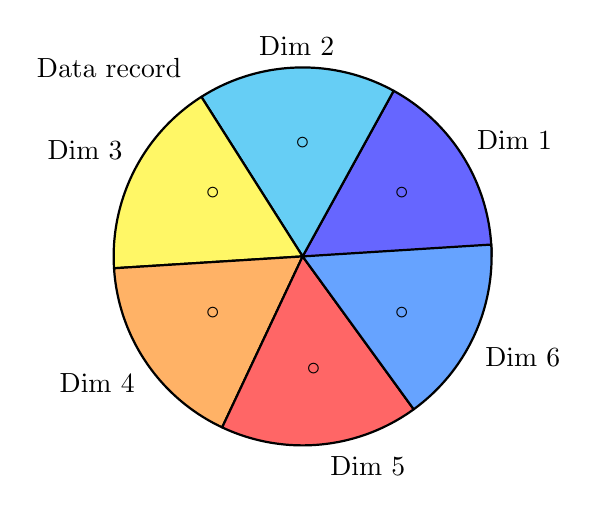
\begin{tikzpicture}[scale=0.8]
		\pie[hide number]{17/Dim 1, 17/Dim 2, 17/Dim 3, 17/Dim 4, 17/Dim 5, 16/Dim 6}
		\node at (1.5, 1) (a) {\tikzmark{t1} $\circ$};
		\node at (-1.5, 1) (b) {\tikzmark{t2} $\circ$};
		\node at (1.5, -0.9) (c) {\tikzmark{t3} $\circ$};
		\node at (-1.5, -0.9) (d) {\tikzmark{t4} $\circ$};
		\node at (0.1, -1.8) (e) {\tikzmark{t5} $\circ$};
		\node at (0, 1.8) (f) {\tikzmark{t6}$\circ$};
		\node at (-3, 3) (f) {Data record \tikzmark{n1}};
	\end{tikzpicture}
	\begin{tikzpicture}[remember picture,overlay]
		\path[draw=black,thick,-]<1-> (n1) -- (t1);
		\path[draw=black,thick,-]<1-> (n1) -- (t2);
		\path[draw=black,thick,-]<1-> (n1) -- (t3);
		\path[draw=black,thick,-]<1-> (n1) -- (t4);
		\path[draw=black,thick,-]<1-> (n1) -- (t5);
		\path[draw=black,thick,-]<1-> (n1) -- (t6);
	\end{tikzpicture}
\end{frame}

\begin{frame}{Laying Out Pixels in Circle Segments}
	To save space and show the connections among multiple dimensions, \\
	space filling is often done in a circle segment.\\
	\centering
	\newcommand{\D}{7} % number of dimensions (config option)
	\newcommand{\U}{7} % number of scale units (config option)

	\newdimen\R % maximal diagram radius (config option)
	\R=3.5cm
	\newdimen\L % radius to put dimension labels (config option)
	\L=4cm
	\newcommand{\A}{360/\D} % calculated angle between dimension axes

	\begin{tikzpicture}[scale=0.7]
		\path (0:0cm) coordinate (O); % define coordinate for origin

		% draw the spiderweb
		\foreach \X in {1,...,\D}{
				\draw (\X*\A:0) -- (\X*\A:\R);
			}

		\foreach \Y in {0,...,\U}{
				\foreach \X in {1,...,\D}{
						\path (\X*\A:\Y*\R/\U) coordinate (D\X-\Y);
						\fill (D\X-\Y) circle (1pt);
					}
				\draw [opacity=0.3] (0:\Y*\R/\U) \foreach \X in {1,...,\D}{
						-- (\X*\A:\Y*\R/\U)
					} -- cycle;
			}

		% define labels for each dimension axis (names config option)
		\path (1*\A:\L) node (L1) {Dim 1};
		\path (2*\A:\L) node (L2) {Dim 2};
		\path (3*\A:\L) node (L3) {Dim 3};
		\path (4*\A:\L) node (L4) {Dim 4};
		\path (5*\A:\L) node (L5) {Dim 5};
		\path (6*\A:\L) node (L6) {Dim 6};
		\path (7*\A:\L) node (L7) {Dim 7};

		% for each sample case draw a path around the web along concrete values
		% for the individual dimensions. Each node along the path is labeled
		% with an identifier using the following scheme:
		%
		% D<d>-<v>, dimension <d> a number between 1 and \D (#dimensions) and
		% value <v> a number between 0 and \U (#scale units)
		%
		% The paths will be drawn half-opaque, so that overlapping parts will be
		% rendered in a composite color.

		% Example Case 1 (red)
		%
		% D1 (Security): 0/7; D2 (Content Quality): 5/7; D3 (Performance): 0/7;
		% D4 (Stability): 6/7; D5 (Usability): 0/7; D6 (Generality): 5/7;
		% D7 (Popularity): 0/7
		\draw [color=red,line width=1.5pt,opacity=0.5]
		(D1-0) --
		(D2-5) --
		(D3-0) --
		(D4-6) --
		(D5-0) --
		(D6-5) --
		(D7-0) -- cycle;

		% Example Case 2 (green)
		%
		% D1 (Security): 2/7; D2 (Content Quality): 2/7; D3 (Performance): 5/7;
		% D4 (Stability): 1/7; D5 (Usability): 4/7; D6 (Generality): 1/7;
		% D7 (Popularity): 7/7
		\draw [color=green,line width=1.5pt,opacity=0.5]
		(D1-2) --
		(D2-2) --
		(D3-5) --
		(D4-1) --
		(D5-4) --
		(D6-1) --
		(D7-7) -- cycle;

		% Example Case 3 (blue)
		%
		% D1 (Security): 1/7; D2 (Content Quality): 7/7; D3 (Performance): 4/7;
		% D4 (Stability): 4/7; D5 (Usability): 3/7; D6 (Generality): 5/7;
		% D7 (Popularity): 2/7
		\draw [color=blue,line width=1.5pt,opacity=0.5]
		(D1-1) --
		(D2-7) --
		(D3-4) --
		(D4-4) --
		(D5-3) --
		(D6-5) --
		(D7-2) -- cycle;

	\end{tikzpicture}
\end{frame}

\begin{frame}{Geometric Projection Visualization Techniques}
	\begin{itemize}
		\item Visualization of geometric transformations and projections of data.
		\item \textbf{Methods}:
		      \begin{itemize}
			      \item Scatter plot and scatter plot matrices.
			      \item Landscapes.
			      \item Projection pursuit technique: \emph{Help users find meaningful projections of multidimensional data.}
			      \item Prosection views.
			      \item Hyperslice.
			      \item Parallel coordinates.
		      \end{itemize}
	\end{itemize}
\end{frame}

\begin{frame}{Scatter Plot Matrices}
	\centering
	\includegraphics[height=6.5cm]{img/scatterplot_matrix.pdf}
\end{frame}

\begin{frame}{Parallel Coordinate Plot}
	\centering
	\vspace{0.5cm}
	\begin{tikzpicture}
		\begin{groupplot}[
				group style={
						group name=iris,
						group size=4 by 1,
						horizontal sep=2cm
					},
				axis y line=left,
				hide x axis,
				width=2cm,
				height=6cm,
				xmin=0,
				xmax=0.5,
				enlarge y limits,
				every axis plot/.append style={opacity=0}
			]

			\nextgroupplot

			\pgfplotsinvokeforeach{0,...,\NumRows} % loop over all rows in table
			{
				% get value in sw column
				\pgfplotstablegetelem{####1}{sw}\of{\iris}%
				% add a coordinate at x=0 and that y-value
				\edef\temp{\noexpand\addplot coordinates {(0,\pgfplotsretval)} coordinate (sl####1);}
				\temp
			}

			\nextgroupplot

			\pgfplotsinvokeforeach{0,...,\NumRows}
			{
				\pgfplotstablegetelem{####1}{sl}\of{\iris}%
				\edef\temp{\noexpand\addplot coordinates {(0,\pgfplotsretval)} coordinate (sw####1);}
				\temp
			}

			\nextgroupplot

			\pgfplotsinvokeforeach{0,...,\NumRows}
			{
				\pgfplotstablegetelem{####1}{pw}\of{\iris}%
				\edef\temp{\noexpand\addplot coordinates {(0,\pgfplotsretval)} coordinate (pl####1);}
				\temp
			}

			\nextgroupplot

			\pgfplotsinvokeforeach{0,...,\NumRows}
			{
				\pgfplotstablegetelem{####1}{pl}\of{\iris}%
				\edef\temp{\noexpand\addplot coordinates {(0,\pgfplotsretval)} coordinate (pw####1);}
				\temp
			}

		\end{groupplot}

		% add labels below
		\foreach \i/\txt in {1/SW,2/SL,3/PW,4/PL}
		\node [below] at (iris c\i r1.south west) {\txt};


		% draw the lines
		% this dataset has three groups of fifty rows each, hence the start/stop values
		\foreach[
			evaluate=\j as \START using int(\j*50),
			evaluate=\j as \STOP using int((\j+1)*50-1),
		] \j/\clr in {0/blue,1/red,2/green}
			{
				\foreach \i in {\START,...,\STOP}
				\draw [color=\clr,opacity=0.5] (sl\i) -- (sw\i) -- (pl\i) -- (pw\i);
			}

	\end{tikzpicture}
\end{frame}

\begin{frame}{Icon Based Visualization}
	\centering
	\begin{itemize}
		\item \textbf{Visualization of the data values as features of icons.}
		\item \textbf{Typical visualization methods:}
		      \begin{itemize}
			      \item Chernoff faces.
			      \item Stick figures.
		      \end{itemize}
		\item \textbf{General techniques:}
		      \begin{itemize}
			      \item Shape coding: \emph{Use shape to represent certain information encoding.}
			      \item Color icons: \emph{Use color icons to encode more information.}
			      \item Tile bars: \emph{Use small icons to represent the relevant feature vectors in document retrieval.}
		      \end{itemize}
	\end{itemize}
\end{frame}

\begin{frame}{Chernoff Faces}
	\textbf{A way to display variables on a two-dimensional surface:}\\
	E.g. let $x$ be eyebrow slant, $y$ be eye size, $z$ be nose length etc.\\
	The figure shows faces produced using $10$ characteristics (head eccentricity, eye size, eye spacing, eye eccentricity, pupil size, eyebrow slant, nose size, mouth shape, mouth size, and mouth opening). Each assigned one of $10$ possible values, generated using \href{https://www.wolfram.com/mathematica/}{Mathematica} (S. Dickson).\\[0.5cm]
	\centering
	\includegraphics[width=4cm]{img/chernoff_faces_construction.pdf}
\end{frame}

\begin{frame}{Stick Figure}
	A census data figure showing age, income, gender, education etc. \\
	A $5$-piece stick figure ($1$ body and $4$ limbs w. different angle/length).\\[0.1cm]
	\centering
	\includegraphics[width=8cm, height=5.2cm]{img/stick_figure.png}\\
	\tiny{Used by permission of G. Grinstein, University of Massachusettes at Lowell.}
\end{frame}

\begin{frame}{Hierarchical Visualization Techniques}
	\centering
	\begin{itemize}
		\item \textbf{Visualization of the data using a hierarchical partitioning into subspaces.}
		\item \textbf{Methods:}
		      \begin{itemize}
			      \item Worlds within worlds.
			      \item Tree maps.
			      \item Cone trees.
			      \item Info cube.
		      \end{itemize}
	\end{itemize}
\end{frame}

\begin{frame}{Worlds Within World}
	\begin{itemize}
		\item Assign the function and two most important parameters to innermost world.
		\item Fix all other parameters at constant values -- draw other (1,2 or 3) dimensional worlds choosing these as the axes.
	\end{itemize}
	\centering
	\includegraphics[width=8cm,height=5.2cm]{img/www.jpg}
\end{frame}

\begin{frame}{Tree Maps}
	\centering
	\begin{itemize}
		\item \textbf{Screen filling method:}
		      \begin{itemize}
			      \item Uses a hierarchical partitioning of the screen into regions depending on the attribute values.
			      \item $x$ and $y$-coordinates of the screen partitioned alternately according to the attribute values.
		      \end{itemize}
	\end{itemize}
	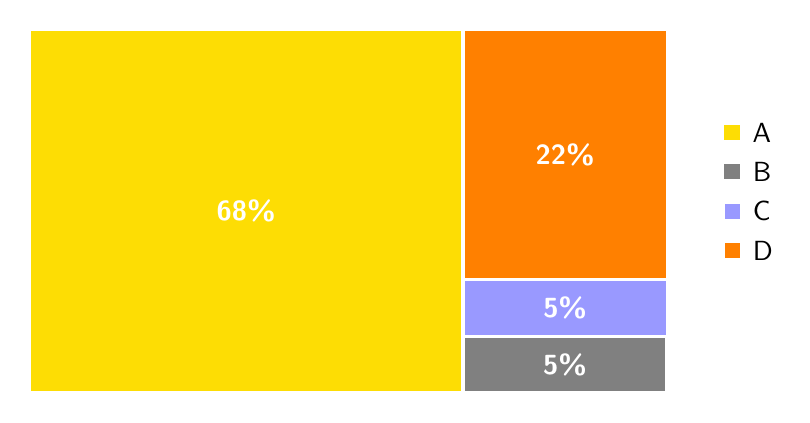
\begin{tikzpicture}[xscale = 1.35, yscale = 0.77,
			font=\sffamily,
			mystyle/.style={draw=white, very thick, text=white, font=\sffamily\bfseries},
		]
		\pie[square,
			style={mystyle},
			color={yellow!80!orange, gray, blue!40, orange},
			text=legend,
		]{68/A, 5/B, 5/C, 22/D}
	\end{tikzpicture}
\end{frame}

\begin{frame}{Tree Map of a File System}
	\centering
	\vspace{0.5cm}
	\includegraphics[width=9cm, height=6cm]{img/treemap_filesystem.png}
\end{frame}

\begin{frame}{Info Cubes}
	\begin{itemize}
		\item $3$D visualization technique:
		      \begin{itemize}
			      \item Hierarchical information is displayed as nested semi-transparent cubes.
			      \item The outermost cubes correspond to the top level data, while the subnodes or the lower level data are represented as smaller cubes inside the outermost cubes, and so on.
		      \end{itemize}
	\end{itemize}
	\vspace{0.2cm}
	\centering
	\includegraphics[width=4cm,height=4cm]{img/infocube.png}
\end{frame}

\begin{frame}{Three Dimensional Cone Trees}
	\centering
	\begin{itemize}
		\item $3$D cone-tree visualization technique:\\
		      works well for up to approx. a thousand nodes.
		\item Build a $2$D circle tree that arranges its nodes in concentric circles centered on the root node.
		\item Overlaps can't be avoided projecting onto $2$D.
		\item G. Robertson, J. Mackinlay, S. Card. "Cone Trees: Animated 3D Visualizations of Hierarchical Information", ACM SIGCHI'91.
	\end{itemize}
	\vspace{0.2cm}
	\includegraphics[width=3cm,height=3cm]{img/threedcone_one.jpg}\hspace{1cm}
	\includegraphics[width=3cm,height=3cm]{img/threedcone_two.jpg}\\
	\tiny{Acknowledgement: \href{ttp://nadeausoftware.com/articles/visualization}{http://nadeausoftware.com/articles/visualization}.}
\end{frame}

\begin{frame}{Visualizing Complex Data and Relations}
	\centering
	\begin{itemize}
		\item \textbf{Visualizing non-numerical data: text and social networks.}
		\item \textbf{Tag cloud: visualizing user-generated tags.}
		      \begin{itemize}
			      \item The importance of tag is represented by font size/color.
			      \item Besides text data, there are also methods to visualize relationships, \\ such as visualizing social networks.
		      \end{itemize}
	\end{itemize}
	\includegraphics[width=7cm,height=4cm]{img/google_news.png}
\end{frame}

\section{Measuring Data Similarity and Dissimilarity}

\begin{frame}{Motivation}
	Similarity and Dissimilarity is inherently important for applications like
	\begin{itemize}
		\item \textbf{Nearest-Neighbor Classification} (c.f. lecture 7).

		      Assign class label to similar objects.

		      Example: spam classification or patient diagnosis.
		\item \textbf{Clustering} (c.f. lecture 8).

		      Cluster customers based on similar properties such as income, age, area of residence).

		      Useful for \textit{marketing} campaigns.

		\item \textbf{Outlier Analysis} (c.f. lecture 9).

		      Cluster data objects to identify outliers.
	\end{itemize}

	\begin{block}{Cluster}
		A \textit{cluster} subsumes data objects that are \underline{similar} to
		each other yet \underline{dissimilar} to data objects of other clusters.
	\end{block}

\end{frame}


\begin{frame}{Similarity and Dissimilarity}
	\begin{columns}
		\begin{column}{0.5\textwidth}
			\textbf{Similarity}
			\begin{itemize}
				\item Numerical measure of how alike two data objects are.
				\item Value is higher when objects are more alike.
				\item Often chosen within the range of $[0,1]$.
			\end{itemize}
		\end{column}
		\begin{column}{0.5\textwidth}
			\textbf{Dissimilarity}
			\begin{itemize}
				\item E.g. distance.
				\item Numerical measure of how different two data objects are.
				\item Lower when objects are more alike.
				\item Minimum dissimilarity is often $0$.
				\item Upper limit varies.
			\end{itemize}
		\end{column}
	\end{columns}

	\begin{alertblock}{Proximity}
		\textit{Proximity} can refer to similarity or dissimilarity.
	\end{alertblock}
\end{frame}

\begin{frame}{Data Matrices and Dissimilarity Matrices}
	\begin{columns}
		\begin{column}{0.5\textwidth}
			\textbf{Data Matrix}

			\begin{itemize}
				\item Stores data objects.
				\item Also called \textit{object-by-attribute structure}.
				\item Each data object is desribed by $m$ attributes.
				\item Having $n$ data objects we have a $n\times m$ data matrix.
			\end{itemize}
			\vspace*{1em}
			\begin{center}
				{$\begin{Bmatrix}
							x_{11} & x_{12} & \cdots & x_{1m} \\
							x_{21} & x_{22} & \cdots & x_{2m} \\
							\vdots & \vdots & \ddots & \vdots \\
							x_{n1} & x_{n2} & \cdots & x_{nm}
						\end{Bmatrix}$ }
			\end{center}
		\end{column}

		\begin{column}{0.5\textwidth}
			\textbf{Dissimilarity Matrix}

			\begin{itemize}
				\item Stores dissimilarity values of data object pairs.
				\item Also called \textit{object-by-object structure}.
			\end{itemize}
			\begin{center}
				{$\begin{Bmatrix}
							0              & 0              & 0              & \cdots & 0      \\
							d(x_{1},x_{2}) & 0              & 0              & \cdots & 0      \\
							d(x_{1},x_{3}) & d(x_{2},x_{3}) & 0              & \cdots & 0      \\
							\vdots         & \vdots         & \vdots         & \ddots & \vdots \\
							d(x_{1},x_{m}) & d(x_{2},x_{m}) & d(x_{3},x_{m}) & \cdots & 0
						\end{Bmatrix}$}
			\end{center}
			with $d(i, j)$ as the measured dissimilarity between two objects $i$ and $j$.

			\textit{Similarity} expressed with $\text{sim}(i,j) = 1 - d(i, j)$.
		\end{column}
	\end{columns}
\end{frame}

\begin{frame}{Proximity Measures for Nominal Attributes}
	Recall: Nominal attributes can take two or more states and values do not follow an order.
	\begin{itemize}
		\item Values can be the same (distance of $0$) or different (distance of $1$).
		\item More options for sets of nominal attributes (variables).
		      \begin{enumerate}
			      \item \textbf{Simple Matching Coefficient} (SMC).
			            \begin{align*}
				            \text{SMC} = \frac{\# \text{of matching attributes}}{\# \text{number of attributes}}
			            \end{align*}
			      \item \textbf{One-Hot Encoding.}

			            Convert nominal attributes to binary attributes,\\ i.e. create one
			            binary attribute for every unique nominal value.
		      \end{enumerate}
	\end{itemize}

	\vspace*{1em}
	\begin{block}{Proximity Measure for Ordinal Attributes}
		Perform \textbf{Integer Encoding}, where every unique value is assigned an integer value.
	\end{block}
\end{frame}

\begin{frame}{Proximity Measure for Binary Attributes}
	\begin{itemize}
		\item Contingency table for binary data that counts matches.
		      \begin{center}
			      \vspace{-2em}
			      \[
				      \text{dasta object}~i\underbrace{
					      \left\{\begin{tabular}{ c | c c c }
						             & $1$   & $0$   & $\sum$    \\ \hline
						      $1$    & $q$   & $r$   & $q+r$     \\
						      $0$    & $s$   & $t$   & $s+t$     \\
						      $\sum$ & $q+s$ & $r+t$ & $q+r+s+t$
					      \end{tabular}\right.}_{\let\scriptstyle\textstyle\substack{\text{data object}~j}}
			      \]
		      \end{center}
		\item Distance measure for \textit{symmetrical} binary variables: $d(x,y) = \frac{r+s}{q+r+s+t}$
		      \note{Symmetrical binary values: each unique value is equally important.}
		\item Distance measure for \textit{asymmetrical} binary variables: $d(x,y) = \frac{r+s}{q+r+s}$
		      \note{Asymmetrical binary values: each unique value is not equally important. Example: Result of disease test.}
		\item Similarity for asymmetrical binary values is called \textit{Jaccard} coefficient and calculated as follows:
		      \begin{align*}
			      \text{sim}(i,j)=\text{jaccard}(i,j)=1-d(i,j)=\frac{q}{q+r+s}
		      \end{align*}
	\end{itemize}
\end{frame}

\begin{frame}{Dissimilarity Between Binary Variables: An Example}
	\begin{center}
		\begin{tabular}{c | c | c | c | c | c | c | c}
			\textbf{Name} & \textbf{Sex} & \textbf{Fever} & \textbf{Cough} & \textbf{Test-$1$} & \textbf{Test-$2$} & \textbf{Test-$3$} & \textbf{Test-$4$} \\\hline
			Bob           & M            & Y              & N              & P                 & N                 & N                 & N                 \\
			Alice         & F            & Y              & N              & P                 & N                 & P                 & N                 \\
			Charlie       & M            & Y              & P              & N                 & N                 & N                 & N                 \\
		\end{tabular}
	\end{center}

	\begin{alertblock}{Note}
		Attribute ``Sex'' is a symmetrical attribute (all values are of equal importance), whereas all remaining attributes are asymmetrical binary attributes.
	\end{alertblock}

	Let values $Y$ and $P$ be equal to $1$ and the value of $N$ be $0$, then we can compute:

	\vspace*{-2em}
	\begin{columns}
		\begin{column}{0.5\textwidth}
			\begin{align*}
				d(\text{Bob}, \text{Alice}) = \frac{0+1}{2+0+1} \approx 0.33 \\
				d(\text{Bob}, \text{Charlie}) = \frac{1+1}{1+1+1} \approx 0.67
			\end{align*}
		\end{column}
		\begin{column}{0.5\textwidth}
			\begin{align*}
				d(\text{Charlie}, \text{Alice}) = \frac{1+2}{1+1+2} = 0.75
			\end{align*}
		\end{column}
	\end{columns}
\end{frame}

\begin{frame}{Standardizing Numerical Data}
	\begin{itemize}
		\item \textbf{$z$-Score:}
		      \begin{align*}
			      z = \frac{x-\mu}{\sigma}.
		      \end{align*}
		\item $x$ is the score to be standardized; $\mu$ ist the population mean; $\sigma$ is the standard deviation.
		\item The distance between the raw score and the population mean in units of the standard deviation.
		\item Negative when the raw score is below the mean, positive else.
		\item \textbf{An alternative way is to compute the mean absolute deviation (MAD):}
		      \begin{align*}
			      \text{MAD}(X = \{x_1,x_2,\ldots,x_n\}) = \frac{1}{n} \sum_{i=1}^{n} \vert x_i - \bar{x} \vert, \\
			      \text{where} \; \bar{x} = \frac{1}{n} \sum_{i=1}^{n}x_i, \; \text{thus} \; z_i = \frac{x_i-\bar{x}}{\sqrt{\frac{1}{n}\sum_{i=1}^{n}(x_i-\bar{x})^2}}.
		      \end{align*}
	\end{itemize}
\end{frame}

\begin{frame}{Example: Data Matrix and Dissimilarity Matrix}
	\begin{itemize}
		\item Data matrix: \\[0.1cm]
		      \begin{tabular}{| c | c | c |}
			      \hline
			      Point & Attribute $1$ & Attribute $2$ \\\hline
			      $x_1$ & $1$           & $2$           \\\hline
			      $x_2$ & $3$           & $5$           \\\hline
			      $x_3$ & $2$           & $0$           \\\hline
			      $x_4$ & $4$           & $5$           \\\hline
		      \end{tabular}\\[0.5cm]
		\item Dissimilarity matrix (with Euclidean distance): \\[0.1cm]
		      \begin{tabular}{| c | c | c | c | c |}
			      \hline
			            & $x_1$  & $x_2$ & $x_3$  & $x_4$ \\\hline
			      $x_1$ & $0$    &       &        &       \\\hline
			      $x_2$ & $3,61$ & $0$   &        &       \\\hline
			      $x_3$ & $2,24$ & $5,1$ & $0$    &       \\\hline
			      $x_4$ & $4,24$ & $1$   & $5,39$ & $0$   \\\hline
		      \end{tabular}\\[0.2cm]
	\end{itemize}
\end{frame}

\begin{frame}{Distance on Numerical Data: Minkowski Distance}
	\vspace{-1.5em}
	\begin{align*}
		d(x,y) = \sqrt[h]{\sum_{i=1}^{n} \vert x_i-y_i \vert^h}
	\end{align*}

	where $x = (x_1,x_2, \ldots, x_n)$ and $y = (y_1,y_2,\ldots,y_n)$ are two $n$-dimensional data objects.

	In fact, this distance induces a norm over real vector space, called $L_n$-norm.

	\begin{block}{Properties of a $L_n$-norm}
		\begin{itemize}
			\item $d(x,y) \geq 0$, positive definiteness.
			\item $d(x,y) = d(y,x)$, symmetry.
			\item $d(x,y) \leq d(x,z) + d(z,y)$, triangle inequality.
		\end{itemize}

		A distance satisfying this properties is called \textbf{metric}.
	\end{block}
\end{frame}

\begin{frame}{Special Cases of Minkowski Distance}
	\begin{columns}
		\begin{column}{0.5\textwidth}
			$h=1$: \textbf{Manhattan Distance}
			\begin{itemize}
				\item Also known as city block, or $L_1$-norm.
				\item E.g. Hamming distance: number of bits that differ in two binary
				      vectors.
			\end{itemize}
			\vspace*{-1.5em}
			\begin{align*}
				d(x,y) = \sum_{i=1}^{n} \vert x_i - y_i \vert
			\end{align*}

			$h=2$: \textbf{Euclidean}
			\begin{itemize}
				\item Also known as $L_2$-norm.
			\end{itemize}
			\vspace*{-1.5em}
			\begin{align*}
				d(x,y) = \sqrt{\sum_{i=1}^{n} (x_i-y_i)^2}.
			\end{align*}
		\end{column}

		\begin{column}{0.5\textwidth}
			$h \rightarrow \infty:$ \textbf{Supremum}
			\begin{itemize}
				\item Also known as $L_{\text{max}}$-norm, or $L_\infty$-norm.
				\item Maximum difference between any attribute of two vectors.
			\end{itemize}
			\vspace*{-1.5em}
			\begin{align*}
				d(x,y) = \lim_{h \rightarrow \infty} \left( \sum_{i=1}^{n} \vert x_i - y_i \vert^{h} \right)^{\frac{1}{h}} = \max_i \vert x_i-y_i \vert.
			\end{align*}
		\end{column}
	\end{columns}
\end{frame}

% TODO: (Dis-)Similarity of data objects with mixed attribute types, c.f. chapter 2.4.6, page 75
% TODO: Cosine Similarity, c.f. chapter 2.4.7, page 77

\section{Summary}

\begin{frame}
	\frametitle{Summary}
	\begin{itemize}
		\item  \textbf{Types of outliers:}
		      \begin{itemize}
			      \item Global, contextual \& collective outliers.
		      \end{itemize}
		\item \textbf{Outlier detection:}
		      \begin{itemize}
			      \item Supervised, semi-supervised, or unsupervised.
		      \end{itemize}
		\item \textbf{Statistical (or model-based) approaches.}
		\item \textbf{Proximity-based approaches.}
		\item \textbf{Not covered here:}
		      \begin{itemize}
			      \item Clustering-based approaches.
			      \item Classification approaches.
			      \item Mining contextual and collective outliers.
			      \item Outlier detection in high dimensional data.
		      \end{itemize}
	\end{itemize}
\end{frame}

\begin{frame}[c]
	\begin{center}
		{\bf Any questions about this chapter?}\\[0.5cm]
		Ask them now or ask them later in our forum: \\\bigskip
		\qrcode{https://www.studon.fau.de/studon/goto.php?target=lcode_OLYeD79h} \\
		\vspace*{0.5cm}
		\faLink\ \url{https://www.studon.fau.de/studon/goto.php?target=lcode_OLYeD79h} \smallskip

	\end{center}
\end{frame}


\end{document}
